\documentclass{standalone}

\usepackage{tikz}
\usepackage{charter}

\tikzset{
  rect/.style={fill=black!10, rounded corners}
}

\begin{document}
  
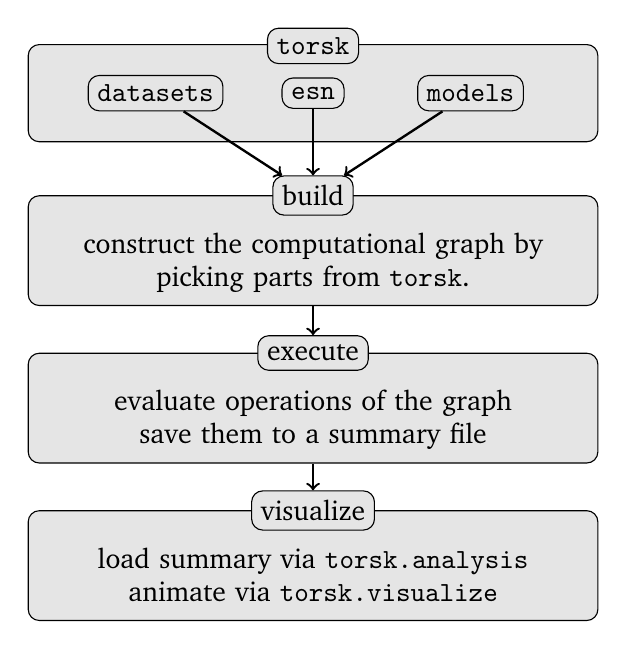
\begin{tikzpicture}
  \node[draw, rect, text width=7cm, text height=1cm] at (0,0) (torsk_frame) {}; 
  \node[draw, rect] at (0, 0.6) (torsk) {\texttt{torsk}};
  \node[draw, rect] at (-2, 0) (data) {\texttt{datasets}};
  \node[draw, rect] at (0, 0) (esn) {\texttt{esn}};
  \node[draw, rect] at (2, 0) (models) {\texttt{models}};

  \node[draw, rect, text width=7cm, text height=0cm] at (0, -2) (build_frame) {
    \begin{center}
    \begin{tabular}{c}
      construct the computational graph by\\ picking parts from \texttt{torsk}.
    \end{tabular}
    \end{center}
  };
  \node[draw, rect] at (0, -1.3) (build) {build};

  \node[draw, rect, text width=7cm, text height=0cm] at (0, -4) (exec_frame) {
    \begin{center}
    \begin{tabular}{c}
      evaluate operations of the graph\\
      save them to a summary file
    \end{tabular}
    \end{center}
  };
  \node[draw, rect] at (0, -3.3) (execute) {execute};

  \node[draw, rect, text width=7cm, text height=0cm] at (0, -6) (vis_frame) {
    \begin{center}
    \begin{tabular}{c}
      load summary via \texttt{torsk.analysis}\\
      animate via \texttt{torsk.visualize}
    \end{tabular}
    \end{center}
  };
  \node[draw, rect] at (0, -5.3) (vis) {visualize};

  \path[draw, ->, line width=0.3mm] (data) edge (build) node {};
  \path[draw, ->, line width=0.3mm] (esn) edge (build) node {};
  \path[draw, ->, line width=0.3mm] (models) edge (build) node {};
  \path[draw, ->, line width=0.3mm] (build_frame) edge (execute) node {};
  \path[draw, ->, line width=0.3mm] (exec_frame) edge (vis) node {};

\end{tikzpicture}

\end{document}
